\documentclass[12pt]{article}
\usepackage[english]{babel}
\usepackage[utf8x]{inputenc}
\usepackage{amsmath}
\usepackage{graphicx}
\usepackage[colorinlistoftodos]{todonotes}
\usepackage{cite}
\usepackage{acro}
\acsetup{first-style=short}
\DeclareAcronym{rest}{
  short = REST ,
  long  = Representational State Transfer ,
  class = abbrev
}
\DeclareAcronym{api}{
  short = API ,
  long  = Application Programming Interface ,
  class = abbrev
}
\DeclareAcronym{tm}{
  short = TM ,
  long  = Trademark ,
  class = abbrev
}
\DeclareAcronym{json}{
  short = JSON ,
  long  = JavaScript Object Notation ,
  class = abbrev
}
\DeclareAcronym{sql}{
  short = SQL ,
  long  = Structured Query Language ,
  class = abbrev
}
\DeclareAcronym{http}{
  short = HTTP ,
  long  = Hypertext Transfer Protocol ,
  class = abbrev
}
\DeclareAcronym{dsl}{
  short = DSL ,
  long  = Domain Specific Language ,
  class = abbrev
}



\begin{document}

	\begin{titlepage}
		\newcommand{\HRule}{\rule{\linewidth}{0.5mm}} % Defines a new command for the horizontal lines, change thickness here
		\center % Center everything on the page
		 
		%	HEADING SECTIONS

		\textsc{\LARGE College of Engineering, Trivandrum}\\[1.5cm] % Name of your university/college
		\textsc{\Large Computer Science and Engineering}\\[0.5cm] % Major heading such as course name
		% \textsc{\large Minor Heading}\\[0.5cm] % Minor heading such as course title
		
\includegraphics[width=5cm]{images/cet_emblem.jpg} 

		%	TITLE SECTION
		\HRule \\[0.4cm]
		{ \huge \bfseries Elastic Search}\\[0.4cm] % Title of your document
		\HRule \\[1.5cm]

		%	AUTHOR SECTION
		\begin{minipage}{0.4\textwidth}
		\begin{flushleft} \large
		\emph{Submitted By:}\\
		Mohammed Nisham K % Your name
		mnishamk1995@gmail.com
		Roll No 39
		\end{flushleft}
		\end{minipage}
		~
		\begin{minipage}{0.4\textwidth}
		\begin{flushright} \large
		\emph{Guide:} \\
		Vipin Vasu % Supervisor's Name
		\end{flushright}
		\end{minipage}\\[2cm]

		%	DATE SECTION
		{\large \today}\\[1cm] % Date, change the \today to a set date if you want to be precise

		%	LOGO SECTION
		\vfill % Fill the rest of the page with whitespace
	\end{titlepage}

	\pagenumbering{roman}
	\tableofcontents
	% \newpage
	\listoffigures
	\newpage
	\printacronyms[include-classes=abbrev,name=Abbreviations]
	\newpage

	\pagenumbering{arabic}

	\renewcommand{\abstractname}{\Large Abstract}
	\begin{abstract}
A search server based on Lucene, Elastic Search is a way to organise data and make it readily accessible. A highly scalable, distributed, full-text search engine. Coded completely in java and published as open source under the terms of Apache Licence, it is the most popular enterprise search engine used by giants on the web like facebook, wikipedia, stumbleupon etc. It includes advances in speed, security (with shield plugin), scalability and hardware efficiency out of the box.


Elastc Search is a tool for querying words, its principal task being to return text similar to a given query and statistical and liguistic analysis of it. A standalone database server, communicable only through RESTful API's, it takes data and optimises the data according to language based searches and stores it in a sophisticated manner. It supports clustering, and multiple shards out of the box. It makes for an excellent tool.
\end{abstract}

	\newpage

	\section{Introduction}
		Conventional relational databases fail to work for bigdata applications. No\ac{sql} addresses this problem. But again it fails to incorporate full text search on the saved database. Another issue is real-timing, conventional database techniques do not ensure a real time implementation, so a search engine database implementation is required which addresses these issues.\cite{mine}

		Elastic Search is an open-source realtime distributed search and analytics engine built as an abstraction layer on top of Apache Lucene \textsuperscript{\ac{tm}}\cite{book}. Lucene is an advanced full text search engine with high performance\cite{lucenesite}. But since Lucene is written as a library, it is available only when working with Java and it is very complex to use.

		Elastic provides an abstraction layer implemented in Java, which uses Lucene internally for its operations, but provides a simple method to access them via \ac{rest}ful \ac{api}'s. Since access to operations is via \ac{rest}ful \ac{api}'s, the usage of Elastic Search does not require coding in java, \emph{ie} it can be used from any language.

		Elastic search is widely used by giants on the web. Facebook, Wikipedia, and Github being examples. It was ranked as the most popular search engine database, outranking competitors like Solr and Sphinx.\cite{dbranking}

	\section{History}
		Shay Banon, started working with Lucene, and finding its interface tricky started building an abstraction layer over it. It was released as an open-source library for Java called Compass.\cite{site}

		Later, working in high performance distributed environments revealed the need for distributed solution to search. So Compass libraries were rewritten from scratch with distributed usage in mind. Making it available to different languages was easy as \ac{json} became an accepted standard of representing complex objects serially and \ac{rest}ful \ac{api}'s the standard interface to access functionality via \ac{http} connections, thus its implementaion, serialisation and deserialisation, being available in all languages
	
	\section{Features}
		Elastic Search provides myriads of features on top of abstraction of and simple interface to Lucene. Some of the features, excluding search are explored here

		\subsection{Document Oriented}
			Elastic search is document oriented. Instead of trying to create columns where the data can fit, the data is stored as a \ac{json} object. Not only that, but each field is indexed for searchability. \emph{ie} instead of searching on rows, searching is done on documents.\cite{book}

			\ac{json} is a format of representing complex objects serially. It is the standard format accepted by almost all languages and conversion to and from \ac{json} can be done easily. Representing a document as \ac{json} instead of a native object makes it serial, thus having the added benefit of being a viable parameter in a \ac{http} request, or a \ac{rest}ful \ac{api}.

			\subsubsection{Index}
			Documents are stored under indices. An index is a name given to a store of data. In actuality it is a collective name representing a group of shards which contain the documents. Indices can be considered as analogous to databases in a relational model. Index\textsubscript{(\emph{noun})} is not to be confused with Index\textsubscript{(\emph{verb})} which means to add a document to an index.

			\subsubsection{Type}
			An Index can have documents of multiple types. A type is a logical grouping of documents that are similar, or have content that have most of their fields common. A type can be compared to a table of a relational model. 

			Each type has its own mapping or schema definition which defines how the fields of the documents of that type must be indexed. For example, a date field would be indexed to allow a range filter to be used on it, while a string field would be indexed for full search capability.

			\subsubsection{Id}
			Each document is indexed with an identification field id. Analogous to a row in relational databases, id can be used to get a document from the database, provided you have the index and the type in which it is stored. 

			Id also helps in routing, or determining which shard the document will be stored in, the details of which are provided in the next section

			\subsubsection{Dynamic Mapping}
			Type mappings are optional, if mappings are not provided explicitly, Elastic tries to guess the mapping of the fields provided based on the first document that it is given to index. String fields map to string type, and a standard analyzer is tacked on it while a field with value like `2014/01/01' would be mapped to a date type.

		\subsection{Sharding}
			A shard can be explained simply as a piece of an Index. An index can have multiple shards and each shard is a fully qualified Lucene Search Engine. Each shard can function independantly from every other shard. A sharded index increases its distributed nature.
			\subsubsection{Distributed Document Store}
				Each document in an index is stored in a single shard. The shard to which the document is mapped can be found by the formula \[ shard = hash(id) \% num\_of\_shards\]. Thus the number of shards in an index is unchangable after creation of the index.

				At index time, a document is routed to one of the shards, all \ac{api}s use the function to compute which shard the document is stored in and forwards the request to the correct shard.
			\subsubsection{Primary and Replica Shards}
				There are two kinds of shards, Primary and Replica. The number of primary shards is fixed at index time, but the number of replica shards can be changed. Primary shards contain indexes of the documents provided. Replica shards are exact copies of primary shards. They are useful for failure mitigation in a clustered environment.

			\subsubsection{Shard working}
				A shard has to index documents in such a way that all fields are searchable \emph{ie} it has to cope with multiple values per field. This is solved by using an inverted index. An \emph{inverted index} can be defined as a mapping from all unique terms in the document to the documents they appear in.
				\begin{figure}[ht]
				\begin{center}
				\begin{tabular}{|c|c|c|c|}
					\hline
					Term & Doc1 & Doc2 & Doc3\\
					\hline
					\hline
					Brown & X &  & X \\
					\hline
					quick & X & X & X \\
					\hline
				\end{tabular} 
				\caption{An inverted index}
				\end{center}
				\end{figure}
				Inverted index can be used to efficiently search through a large document set to find words matching the query term.

				The inverted index once stored is immutable, it cannot be changed. This is useful since no locking mechanism needs to be implemented and the data can be accessed by multiple users without fear of change. Morover it decreases query time, since once loaded into memory, this index never changes and thus queries can be served from memory.

				\begin{figure}[ht]
					\centering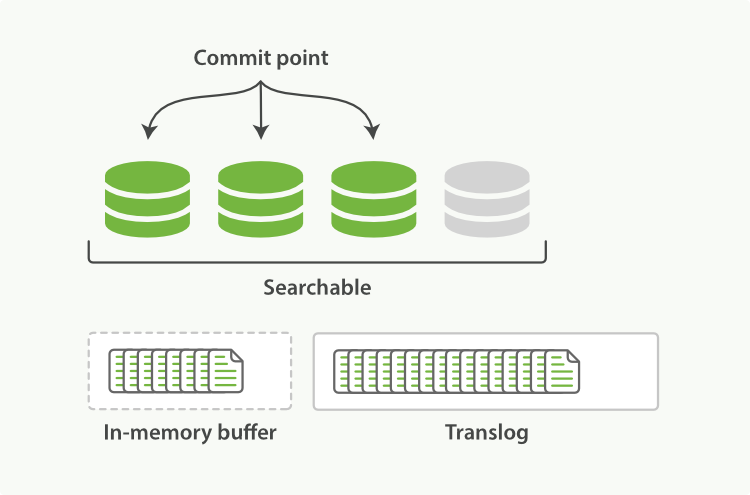
\includegraphics[width=10cm]{images/inside_shard}
					\caption{Inside a shard}
				\end{figure}

				The problem with immutable index is that its immutable, So new indexes can't be saved. This is solved by using multiple indices, namely segments. So a shard can be viewed as a number of segments.A commit point file, tracks all the segments available in the shard. Adding a new document should not be as hard as reindexing an entire segment, so newer indexes are saved in an In-memory buffer, and the In-memory buffer is made searchable as well, when the buffer fills, a new segment is created with the data in the buffer and the buffer is cleared. Old segments may be combined to create larger segments during this time. This operation is known as a refresh and by default Elastic does it every second. Segments and In-memory buffer are used together to get the best worlds.

				The solution above does not protect In-memory buffer against a power failure, to cope with it, a translog is kept in the disk which is updated for each operation on the In-memory buffer. If a shard fails, on restart, the operations in the translog are done to reinstate the In-memory buffer. In contrast to refresh, a flush operation writes the segments to disk and ensures that the segments are written before proceeding or does an fsync operation. Flush clears the translog, since the data is available in disk. By default Elastic flushes every thirty minutes.

		\subsection{Clustering}
			Elastic Search is built to work in a distributed environment, distribution is achieved to some extent using shards, but the real power of elastic comes from clusters. A cluster is a group of nodes working together. Tasks are delegated between the nodes and node acceptance and failure recovery are done automatically. Clustering is done autonomously by Elastic Search with little involvement from the user. Adding new nodes to the cluster, removing nodes, or resharing of shards on node failure are all possible with clustering.

			\subsubsection{Node}
				A node is an instance of an Elastic Search server, capable of handling requests. A node may contain primary and replica shards.A primary shard and its replica are never kept in the same node as a node failure would elimate both. Users can communicate with any node in the cluster. All nodes know the location of each document and can forward the request to the correct node.\cite{ijsr}

			\subsubsection{Cluster Health}
				Cluster health is a measure of safety a cluster has from failure, it is represented as one of three colors, red, yellow or green. Cluster health is calculated in terms of the activeness of primary and replica shards.

				\begin{itemize}
				\item A \textbf{green} cluster health implies that all primary shards and replica shards are active
				\item A \textbf{yellow} cluster health implies that all primary shards are active but not all replica shards are active
				\item A \textbf{red} cluster health implies that not all primary shards are active
				\end{itemize}

			\subsubsection{Horizontal Scaling}
				One of the main motivations of clustering is to increase the througput or decreasing request serve time. Scaling can be done for achieving it. Normally scaling is done vertically by increasing the resources available to program. But horizontal scaling always caps out due to availability of resources and the cost of horizontal scaling will be exponential.

				Another approach that becomes possible with clustering is horizontal scaling. In horizontal scaling, instead of increasing performance in the node, a new node is added. Horizontal scaling has the advantage of being easy, starting another node is the only work involved. Also cost of horizontal scaling increases linearly, so much lower costs can be achieved

			\subsubsection{Failure Recovery}
				The intention behind clustering is to recover in case of a failure without data loss. In a cluster with many nodes, the primary and replica shards are shared between the nodes, with no primary or its replica shard in the same node. When a node dies, and a primary shard is gone, then a replica shard gets promoted to master and the database functions normally.

				\begin{figure}[ht]
					\centering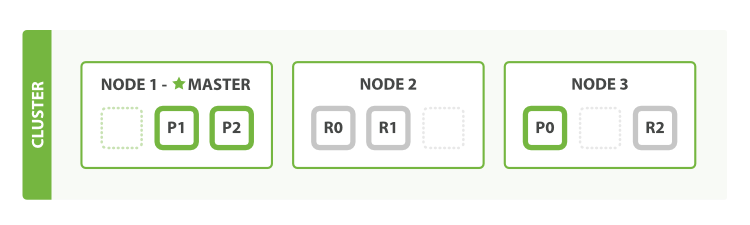
\includegraphics[width=10cm]{images/cluster}
					\caption{A sample cluster}
				\end{figure}

			\subsubsection{Master Node}
				In each cluster, one node is chosen as master which does all cluster level operations. Inviting new nodes into the cluster, polling for new nodes, removing nodes on failure or exit, redistributing primary and replica shards among the nodes on failure of a node are some of the tasks that a master node is assigned. When a master node dies, then another node in the cluster is automatically promoted to master.

				Indexing requests arrive at the master node and it forwards the request to the node which has the primary shard to which the document maps to. The node updates its primary shard and then gives a request to all replica shards to update their content as well. In contrast a get query can be serviced by any node.
				\begin{figure}[ht]
					\centering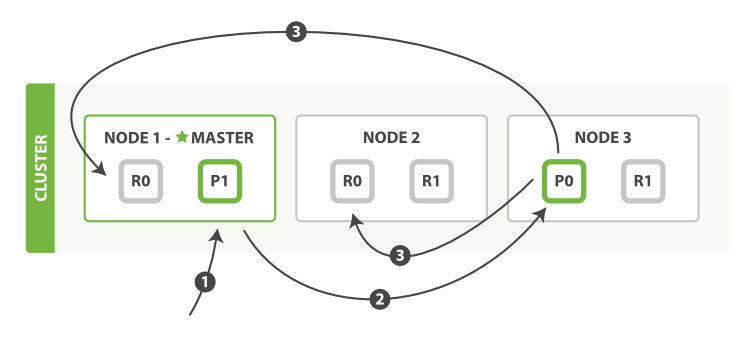
\includegraphics[width=10cm]{images/cluster_data}
					\caption{Request routing in a cluster}
				\end{figure}

			\subsubsection{Autonomy}
				Clusters are completely autonomous, user involvement limits to starting of the node. When a node is started, it automatically identifies any available cluster it can join to and the master in the cluster adds it. If no cluster is found, the node becomes a master and becomes part of a single node cluster. All this happens without the interation of the user. As far as the user is concered, there is no difference between a single node cluster and a multi node cluster save for a decrease in time taken for the request

		\subsection{Mapping and Analysis}
			Elastic provides powerful methods to customize how the inverted index is to be built. They are collectively known as analyzers

			\subsubsection{Analyzers}
				Analyzers are used to determine the words to index, and the ones to discard and the form of the words to index. Stemmers can be used on the words. They can be split on non whitespace regions, and common words can be ignored. These operations are done by an analyzer. By default Elastic uses the standard analyzer, which splits tokens on whitespaces and punctuations, does no stemming and no words are ignored. It can be changed to process languages by using language specific analyzers. Analyzers are a combination of character filter, tokenizer, token filter, and stemmer.

			\subsubsection{Character Filter}
				A character filter filters characters in a field. For example, we could choose to replace all instances of `\&' with and. We might want to make a string consistently encoded, and would use character substitions for the same. Example, ``' and `'' are two types of single quotes which may be replaced by a single type. They are done to increase search effiency by increasing the number of documents matching.

			\subsubsection{Tokenizer}
				Tokenizer decides where each token begins and ends and splits a string into tokens. The default tokenizer splits on whitsespaces and punctuations. This can be altered to suit the need. Tokenizers decide the number of tokens formed from a string.

			\subsubsection{Token Filter}
				Token filters are used to eliminate words that are common. They decide on which tokens to index, and which tokens to eliminate. For example, words like `the', `an' etc could be eliminated from the index, making search faster and more relevant. 

 		\subsection{Aggregations}
				Similar to the GROUP BY commands in \ac{sql}, Aggregation commands are used to provide data over a set of values. This is useful in analysis of data, and for other simpler uses as well. Aggregations are done using buckets and metrics which have a composable syntax and can be combined to create complex queries.

			\subsubsection{Buckets}
				Bucket is a collection of documents that meet a certain criterion.\cite{book} They partition documents based on criteria, it can be thought of as the group by column in relational database. As aggregation proceeds, the values in a document are checked to see if they should be added to the bucket.

			\subsubsection{Metrics}
				Buckets are a means to an end, buckets are usually found to do some calculations on the grouped documents, and these calculations are called metrics. Count, max and min are examples of metrics.

			\subsubsection{Combinations}
				Buckets and metrices can be combined in any way and can even be nested since the composable syntax allows the query to be assembled in various ways. This can then be used in conjunction with queries or filters written in query \ac{dsl}. This allows us to run a query or a filter and run aggregations on the result returned by the query.

		\subsection{Concurrency}
			Elastic Search aims to be distributed. In a distributed system concurrency plays an important role in determining speed with which queries are processed.A good implementation of a distributed system will be as concurrent as possible. 

			\subsubsection{Optimistic Concurrency Control}
				Elastic handles concurrency using \emph{optimistic concurrency control}. It assumes that conflicts are unlikely to happen during indexing operations and does not block operations\cite{book}. But if the document changes between reading and writing the update fails and it is upto the application to decide how to handle a failure. 

			\subsubsection{Metafield \_Version}
				All update and delete operations are done on the primary shard and then propagated to all the replica shards. Since all operations in Elastic are asynchronous and concurrent, the updates may arrive out of order. To ensure that a newer version of the document does not get overwritten by an older version, Elastic uses a metafield called \_version. A document cannot be updated by another document which has equal or lower \_version field. This also solves concurrency since concurrent updates would have the same \_version number.

	\section{Search}
		The most powerful feature of Elastic is its ability to index all fields in a document and then return results based with full text search on these fields, as opposed to a normal No\ac{sql} implementation.

		\subsection{Distributed Search}
			Search requires a more complicated execution model than indexing because we don’t know which
			documents will match the query: they could be on any shard in the cluster. A search
			request has to consult a copy of every shard in the index or indices we’re interested in
			to see if they have any matching documents.
			
			Results from multiple shards must be combined into a single sorted list before the search API can return a	“page” of results. For this reason, search is executed in a two-phase process called query then fetch.

			\subsubsection{Query Phase}
			During the initial query phase, the query is broadcast to a shard copy (a primary or
			replica shard) of every shard in the index. Each shard executes the search locally and
			builds a priority queue of matching documents. All the returned queues are analyzed and single priority queue of required size is created.
				\begin{figure}[ht]
					\centering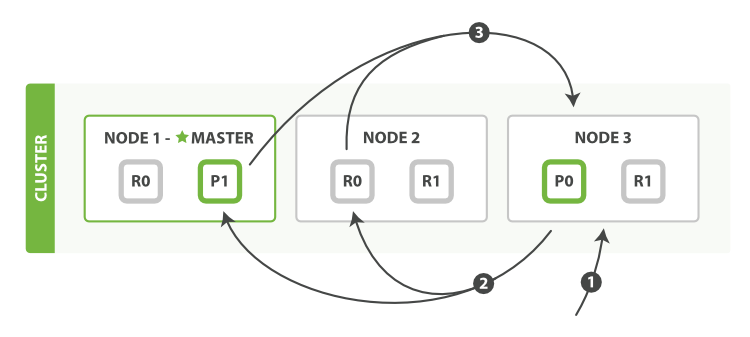
\includegraphics[width=10cm]{images/query_phase}
					\caption{Query phase in distributed search}
				\end{figure}

			\subsubsection{Fetch Phase}
			The query phase identifies which documents satisfy the search request, but the documents aren't retrieved. It is done in fetch phase. Using a multiget request, matching documents are retrieved and an enriched version of the priority queue is formed which is then sent back to the user.
				\begin{figure}[ht]
					\centering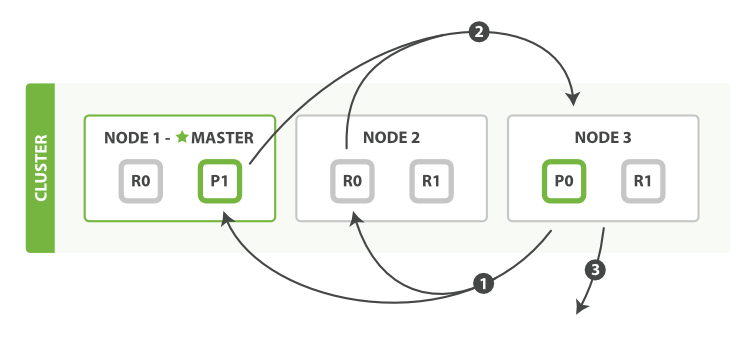
\includegraphics[width=10cm]{images/fetch_phase}
					\caption{Fetch phase in distributed search}
				\end{figure}

		\subsection{Relevance Score}
			Databases that deal purely in structured data (such as dates, numbers, and string
			enums) have it easy. they just have to check whether a document (or a row, in a relational database) matches the query.

			While Boolean yes/no matches are an essential part of full-text search, they are not
			enough by themselves. Instead, the relevance of each document to the query is to be found as well. Full-text search engines have to not only find the matching documents,
			but also sort them by relevance.

			For a query, All matching documents are found, their relevance is found and then they are sorted by it. For this end, there should be a relevance score field for each retrieved document and this is stored in the metadata \_score field. Relevance is affected by the following factors

			\subsubsection{Term Frequency}
				More the term appears in a document, more relevant the term is. For example, A document talking about foxes, would have the term fox repeated throughout. Documents with more term frequency will have a higher relevance score

			\subsubsection{Inverse Document Frequency}
				While term frequency was limited to a single document, inverse document frequency goes beyond and analyses all documents in an index. Terms that are common not only in a single document but also in other documents in the index would rarely be relevant. Terms like `the' and `and' would match this criteria. Hence those terms are given less priority and count less in score calculation. While documents with words that are uncommon across the index are given higher scores.

			\subsubsection{Field Length Normalisation}
				It can be stated simply as, The shorter the field, the more important it is. A title field would be shorter than a body field, so a query matching a title field is given higher score than a query matching the body field. 

			\subsubsection{Boost}
				Druing search or index, individual fields can be boosted to count more towards relevance score. An example would be a tag field. Boosting a tag field ensures that a document is matched when any of tags match. 
	% \nocite{*}
	\newpage
	\bibliography{../common/seminar}
	\bibliographystyle{ieeetr}
\end{document}